\documentclass{standalone}
\usepackage{pgfplots}
\pgfplotsset{compat=1.18}
\usepgfplotslibrary{colorbrewer}
\pgfplotsset{cycle list/Set1-6}

\begin{document}

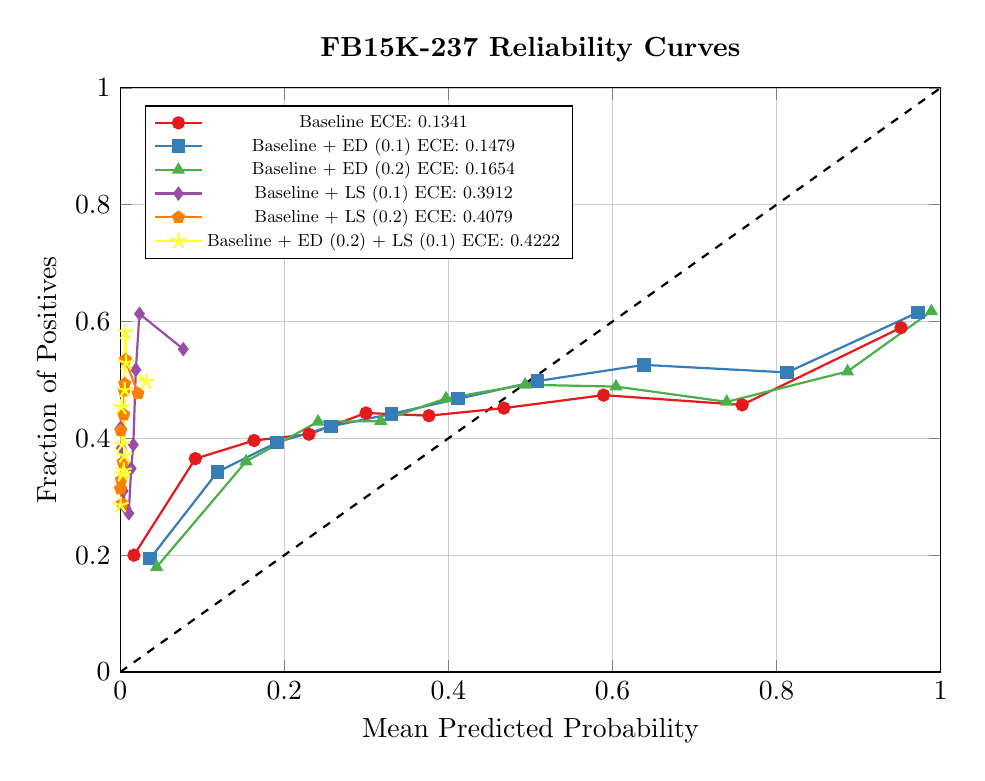
\begin{tikzpicture}
\begin{axis}[
    title={\textbf{FB15K-237 Reliability Curves}},
    xlabel={Mean Predicted Probability},
    ylabel={Fraction of Positives},
    xmin=0, xmax=1,
    ymin=0, ymax=1,
    xtick={0, 0.2, 0.4, 0.6, 0.8, 1.0},
    ytick={0, 0.2, 0.4, 0.6, 0.8, 1.0},
    legend pos=north west,
    legend style={nodes={scale=0.7, transform shape}, font=\small},
    grid=both,
    grid style={line width=.1pt, draw=gray!20},
    major grid style={line width=.2pt, draw=gray!40},
    width=12cm,
    height=9cm,
    cycle list name=Set1-6
]

% Perfectly Calibrated Line
\addplot [color=black, dashed, line width=0.8pt, forget plot]
    coordinates {(0,0)(1,1)};

% Model 1: Baseline
\addplot+[mark=*, thick] coordinates {
    (0.01665991, 0.20004885) (0.0915501, 0.36525776) (0.16314514, 0.39628634) (0.22997979, 0.4070364) 
    (0.29957612, 0.44344002) (0.37629192, 0.43879795) (0.46759511, 0.45174688) (0.58913148, 0.47397997) 
    (0.75807034, 0.45725452) (0.9517584, 0.58954312)
};
\addlegendentry{Baseline ECE: 0.1341}

% Model 2: Baseline + ED (0.1)
\addplot+[mark=square*, thick] coordinates {
    (0.0363344, 0.19394235) (0.11852607, 0.34253604) (0.1911488, 0.39311019) (0.25702976, 0.4207183) 
    (0.33049196, 0.44172978) (0.4116278, 0.46762766) (0.50859403, 0.4981676) (0.63842097, 0.52577571) 
    (0.81277195, 0.51282678) (0.9723146, 0.61553493)
};
\addlegendentry{Baseline + ED (0.1) ECE: 0.1479}

% Model 3: Baseline + ED (0.2)
\addplot+[mark=triangle*, thick] coordinates {
    (0.04440312, 0.17977528) (0.15332931, 0.36037137) (0.24107382, 0.42853653) (0.31759054, 0.4295138) 
    (0.39709684, 0.46836062) (0.49352566, 0.49181529) (0.60428001, 0.48863914) (0.73930518, 0.46249695) 
    (0.88656463, 0.51453701) (0.98876591, 0.61748901)
};
\addlegendentry{Baseline + ED (0.2) ECE: 0.1654}

% Model 4: Baseline + LS (0.1)
\addplot+[mark=diamond*, thick] coordinates {
    (0.0004922, 0.41817294) (0.00136182, 0.38309309) (0.00350409, 0.30979721) (0.00711733, 0.27925727) 
    (0.01043486, 0.27168336) (0.01330828, 0.34839971) (0.01593354, 0.38895676) (0.01899207, 0.51746885) 
    (0.02339561, 0.61324212) (0.07681628, 0.55276014)
};
\addlegendentry{Baseline + LS (0.1) ECE: 0.3912}

% Model 5: Baseline + LS (0.2)
\addplot+[mark=pentagon*, thick] coordinates {
    (0.00026047, 0.3136297) (0.00058063, 0.41338871) (0.0013168, 0.32860982) (0.00226386, 0.28805277) 
    (0.00330721, 0.35890545) (0.00418406, 0.44050818) (0.00483144, 0.48130955) (0.00541067, 0.49328121) 
    (0.00626516, 0.53457122) (0.02161047, 0.47655105)
};
\addlegendentry{Baseline + LS (0.2) ECE: 0.4079}

% Model 6: Baseline + ED (0.2) + LS (0.1)
\addplot+[mark=star, thick, mark size=3pt] coordinates {
    (0.0003858, 0.28553981) (0.00109858, 0.4532128) (0.0022893, 0.38895676) (0.00342556, 0.3383826) 
    (0.00425036, 0.34449059) (0.00491393, 0.37038847) (0.00552733, 0.48228683) (0.00622427, 0.58148058) 
    (0.00712705, 0.52919619) (0.03136405, 0.49682462)
};
\addlegendentry{Baseline + ED (0.2) + LS (0.1) ECE: 0.4222}

\end{axis}
\end{tikzpicture}

\end{document}